\section{INTRODUCTION}
\label{INTRODUCTION}
Anomaly detection problems have a great importance in industrial applications, because anomalies usually represent faults, failures or the emergence of such.
To detect these automatically, advanced analytic algorithms, including machine learning- and deep learning-based, can be applied.
In this work, we investigate deep neural network performances in providing hindsight in oil pipeline diagnostics.
This system spans over thousands of kilometers, which makes manual inspection very costly and sometimes impossible.
The damage of pipelines that transport petroleum and gas products lead to severe environmental problems.
Eliminating breakthroughs and their consequences is expensive.
To avoid accidents, it is recommended to improve diagnostics quality and to increase the frequency of in-line-inspection (ILI) tools deployment.
ILI tools, also referred to as pipeline inspection gauges (Fig.~\ref{ris:ili}), use Hall effect for measuring localized Magnetic Flux Leakage (MFL) intensity along the pipe wall. While moving along the pipe gauge inspects the wall and detects the magnetic field leaks. MFL technique is the most common approach for oil and gas pipelines nondestructive testing nowadays.
\begin{figure}[ht]
	\center{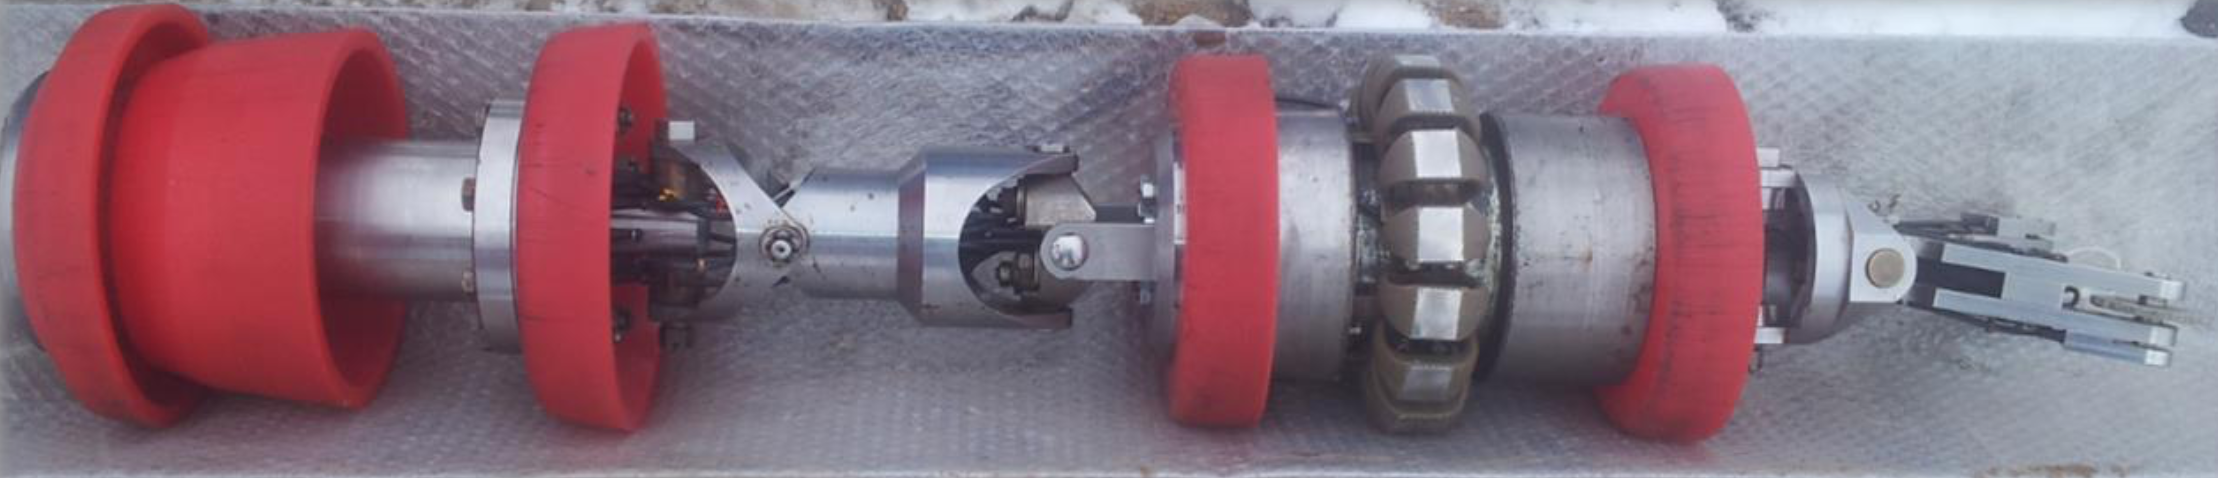
\includegraphics[scale=0.35]{pictures/ili.png}}
	\caption{In-line-inspection tool}
	\label{ris:ili}
\end{figure}
The data collected during the inspection can be further analyzed for main diagnostics problems solving: damage and defects detection, their localization, diagnosis or defects classification.
Analysis results are useful for assets managing and repair priorities determination.

There are three main classes of data that are attended to by diagnostics personnel.
They are presented in Fig.~\ref{ris:classes}.
Some other classes of data (pipe tee, bend) are out of the scope of this work just like different classes of defects.
\begin{figure}[ht]
	\center{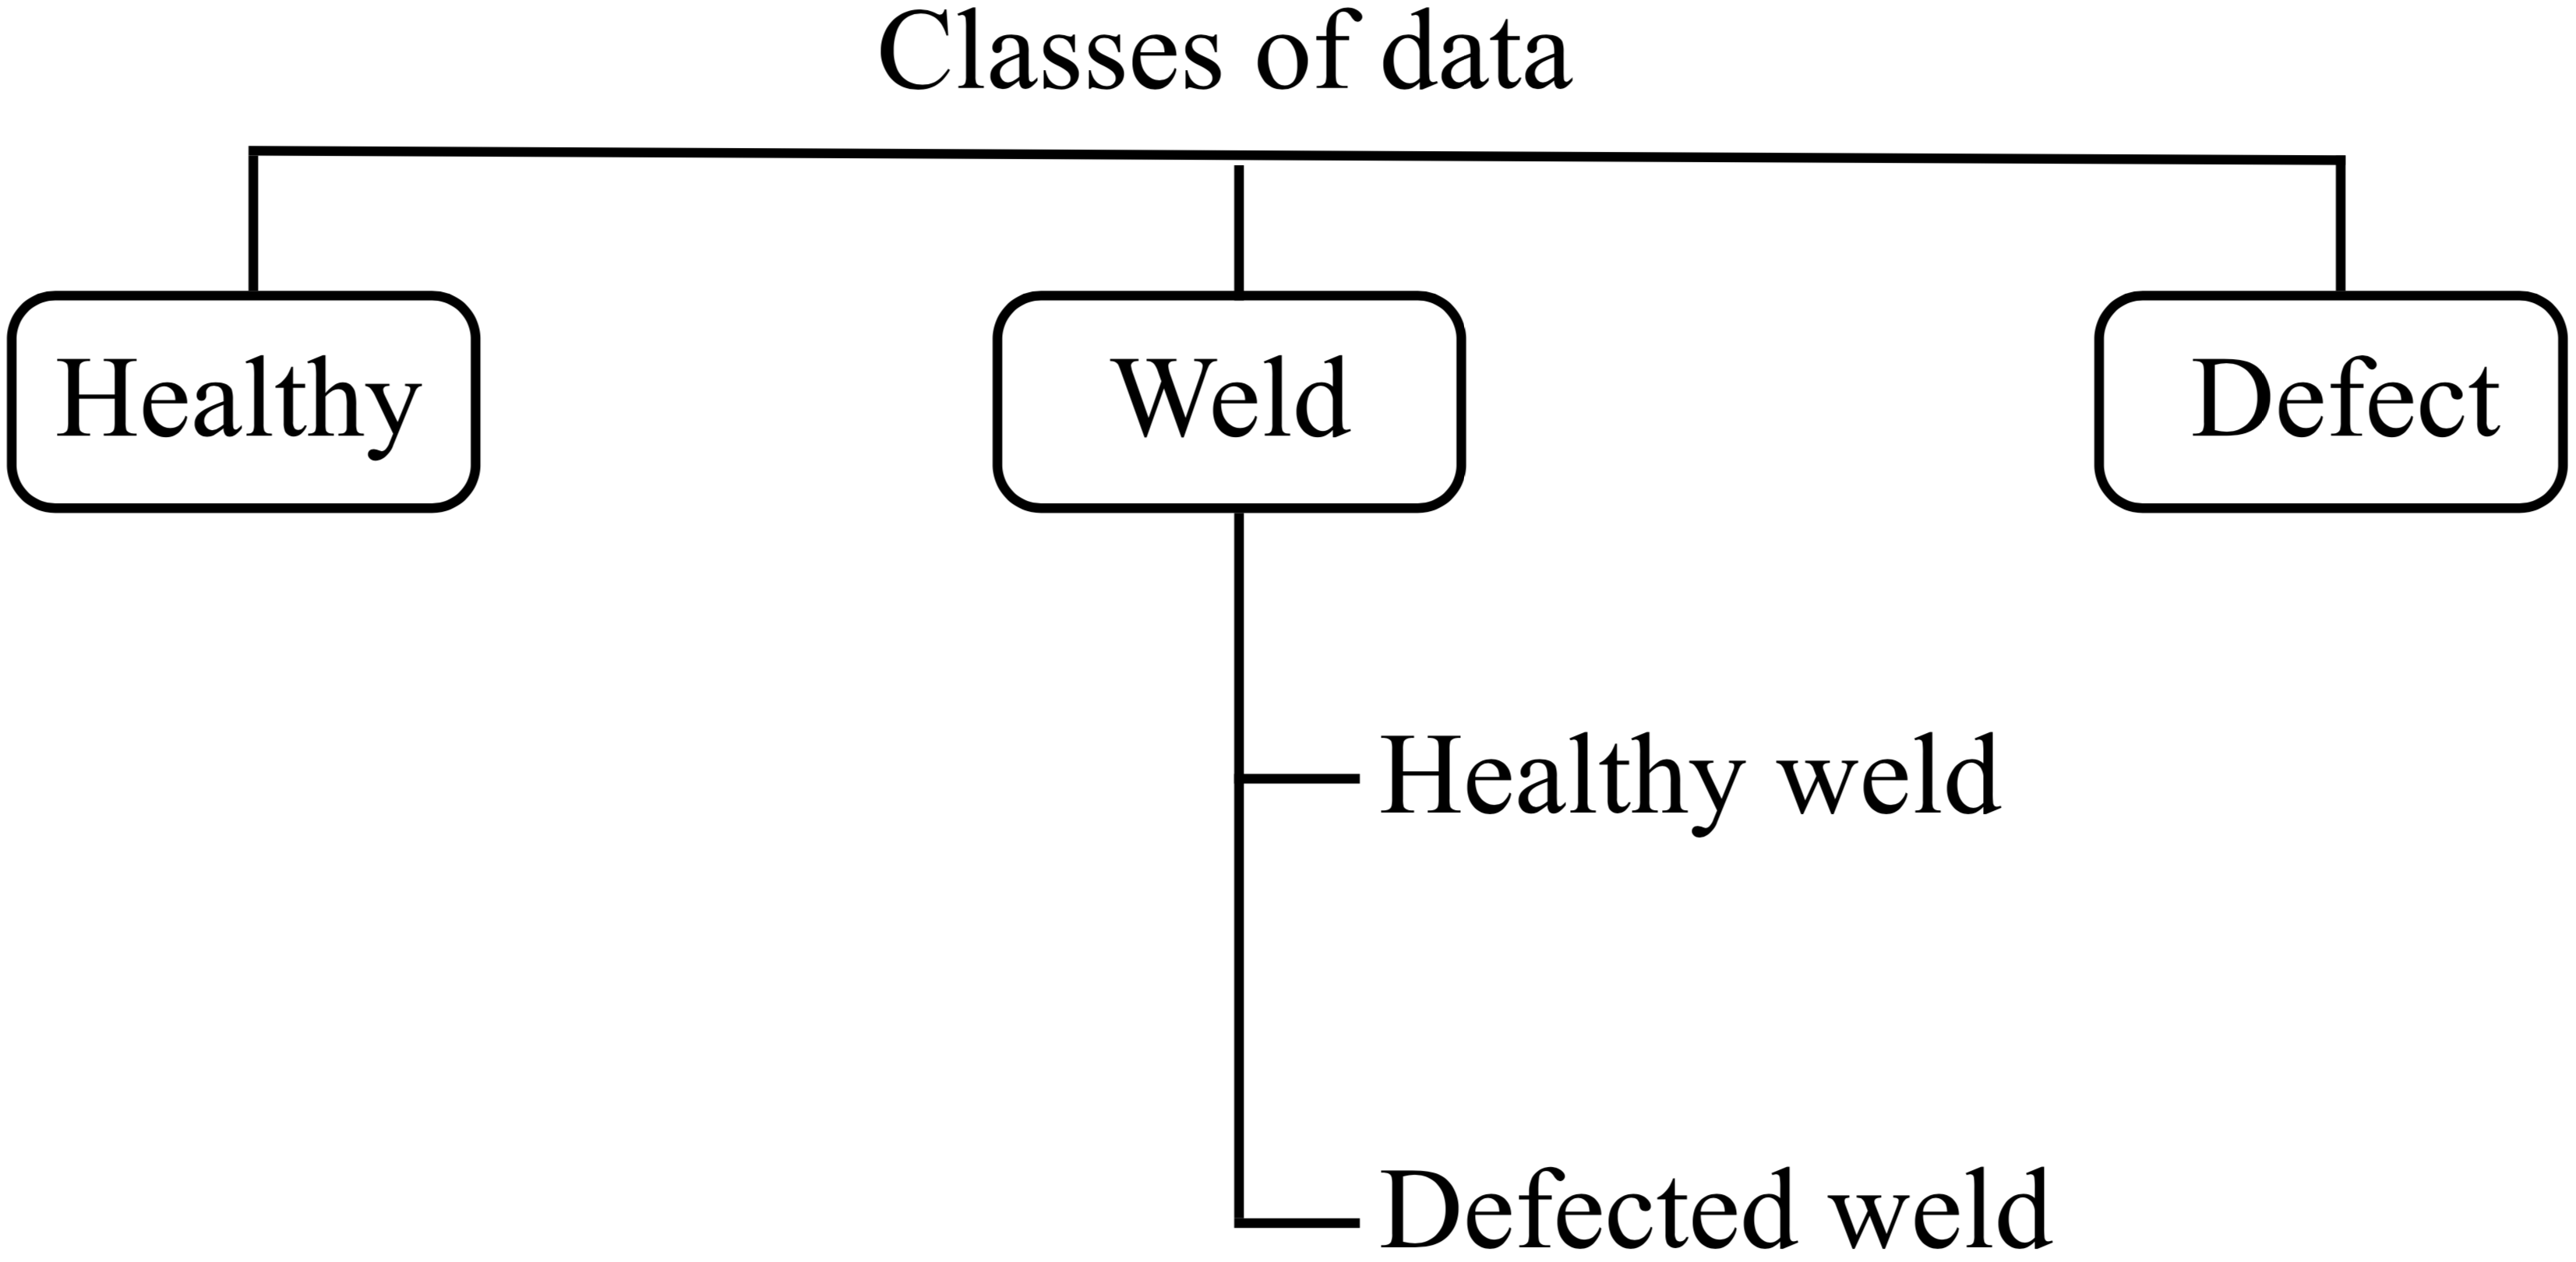
\includegraphics[scale=0.2]{pictures/classes.png}}
	\caption{Image classes that are distinguished in the work}
	\label{ris:classes}
\end{figure}

The rest of the paper is devoted to appraising computer vision (CV) techniques proficiency in oil pipeline diagnostics application.

